One solution to the significant term mismatch between the query and the relevant documents is query expansion, which has been effective in many retrieval tasks. The idea of QE is to add more terms to the original user's query to increase the probability of matching of the query terms with relevant documents, with the objective of improving retrieval effectiveness. The expansion terms can be selected from a feedback process~\citep{cao2008selecting}, or from external sources such as Wikipedia, or dictionaries. Original queries should be expanded by good terms, unless it can lead to retrieval of non-relevant documents.
\paragraph{Feedback-based QE}
\ \\
An initial query can be expanded using a feedback from users-\textit{relevance feedback}-or automatically from top $ k $ ranked retrieved documents, assuming they are relevant to the query-\textit{pseudo relevance feedback}. Getting feedback from  users needs user studies and interaction that is far from our research, so we just explain pseudo relevance feedback in this section. \\\\
\textbf{Pseudo Relevance Feedback (PRF)} 
\ \\
PRF is a standard technique to enrich the initial query with additional terms from the top ranked documents from an initial retrieval run under the assumption that these documents are relevant.
\begin{figure}[htpb]
   \centering
   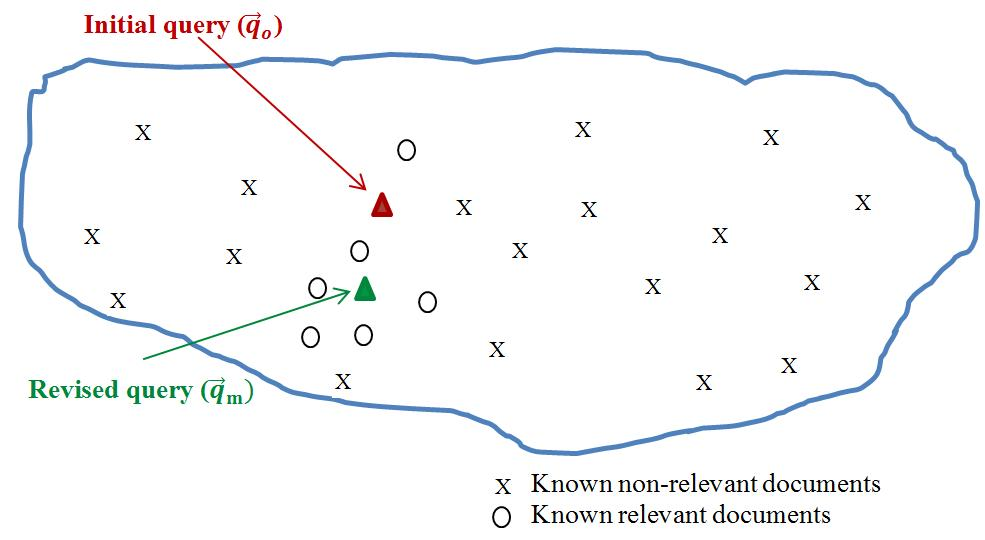
\includegraphics[width=0.65\textwidth,height=50mm]{figs/rocchio.jpg}
   \caption{Rocchio algorithm for relevance feedback. Some documents have been labelled as relevant and non-relevant and the initial query vector is moved in response to this feedback~\citep{manning2008introduction}.}  
   \label{fig:rocchio} 
\end{figure}
\FloatBarrier 
\noindent
The \textit{Rocchio} algorithm is used to modify the query by the partial knowledge of known relevant and non-relevant documents; the goal is to make the query closer to the centroid of the relevant documents but further from irrelevant documents (figure \ref{fig:rocchio}). The modified query, $ \vec{q}_m $ is:
%\[ 
\begin{equation}
\label{eq:rocchio}
 \vec{q}_{m} = \alpha  \vec{q}_{0} + \beta\frac{1}{|D_{r}|}\sum\limits_{\vec{d_{j}}\in D_{r}} \vec{d_{j}} - \gamma\frac{1}{|D_{nr}|}\sum\limits_{\vec{d_{j}}\in D_{nr}} \vec{d_{j}}
  \end{equation}
 %\tag{2.1}\label{eq:rocchio}
 %\]  
where $ q_{0} $ is the original query vector, $ D_{r} $ and $ D_{nr} $ are the set of known relevant and non-relevant documents respectively, and $ \alpha $, $ \beta $, and $ \gamma $ are weights attached to each term. These control the balance between trusting the judged document set versus the query: if we have a lot of judged documents, we
would like a higher $ \beta $ and $ \gamma $~\citep{manning2008introduction}. 
\\\\
\textbf{Predicting the effectiveness of feedback documents or terms } 
\ \\
Distinguishing between good expansion terms and bad ones only based on their distribution (extract the most frequent terms) in the feedback documents and in the whole collection (extract the most specific terms in the feedback documents) is not sufficient. Supervised learning methods for term selection-it is considered as a term classification problem to separate good expansion terms from others directly according to their potential impact on the retrieval effectiveness-helps in this regard. Any classifier can be used to classify terms or feedback documents such as: Suport Vector Machines(SVM)~\citep{cao2008selecting}, Na\"ive Bayes and Logistic Regression~\citep{he2009finding}. 

\paragraph{QE by External Resources}
\ \\
The most common form of query expansion is global analysis, using some form of thesaurus such as dictionaries, WordNet, Wikipedia, and etc. For each term $ t $ in a query, the query can be automatically expanded with synonyms and related words of $ t $ from the thesaurus. Use of a thesaurus can be combined with ideas of term weighting: for instance, one might weight added terms less than original query terms~\citep{manning2008introduction}.